\begin{center}
	\underline{\Large\scshape\bfseries \dytema}
\end{center}
%\markright{INFORME LABORATORIO Nº 05}
%-------------------------------------------------------------------------------------------
\section{Objetivos}
\begin{enumerate}[label=\itemcirccz{azzul}{\arabic*},itemsep=2pt,partopsep=6pt]
	\item Conocer las formas de electrización.
	\item Explicar en que consiste las formas de electrización.
	\item Manejar los instrumentos.
\end{enumerate}

%==========================================================================================
\section{Fundamento teórico}
\subsection{Carga Eléctrica}
Para tener más en claro que es la carga eléctrica el \textbf{Dr\@. Roberto
	Pereira Arroyo} nos indica que \emph{``La Carga Eléctrica son partículas
	subatómicas que se relacionan unas con otras y se hacen con cargas positivas y
	negativas''}, entonces diremos que dichas partículas positivas y neutras se
encontraran en el centro (núcleo) es decir el núcleo de la partícula mientras
los electrones estarán alrededor de la partícula con carga negativa.
\begin{figure}[H]
	\centering
	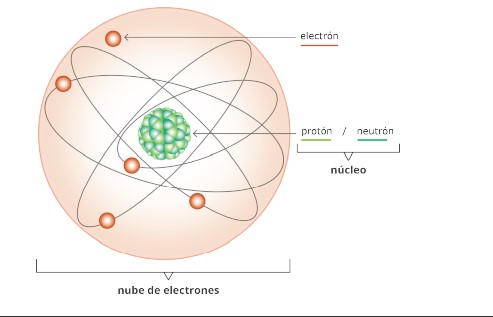
\includegraphics[width=12.5cm]{Images/img1.jpg}
	\caption{Modelo del átomo.}\label{Fig:fg1}
\end{figure}

\sdconditions[12cm]{azzul}{Donde:}{%
	\begin{tabular}{lcl}
		Protón   & \@: & $p^+$                 \\
		Electrón & \@: & $e^-$                 \\
		Neutrón  & \@: & $n$ (no tiene cargas)
	\end{tabular}
}
%==========================================================================================
\subsection{Fomas de Electrización}
\subsubsection{Por Frotamiento}
La electrización por frotamiento según Jorge Humberto Dueñas Rocha ``se
caracteriza por producir cuerpos electrizados con cargas opuestas. Esto ocurre
debido a que los materiales tienen diferente capacidad para retener y entregar
electrones'', en consecuencia, se da cuando dos cuerpos con cargas opuestas ya
sea uno con carga positiva y el otro con carga negativa estos se atraerán al
acercarse y cambiaran de carga haciedno que un cuerpo atraiga al otro cuerpo.
% ------------------------------------------------------------------------------------------
\subsubsection{Por Contacto}
Definiendo la forma que ``un cuerpo eléctricamente neutro aislado, se pone en
contacto con otro cuerpo electrizado o cargado, este le transferirá carga al
cuerpo neutro, ya sea entregándola o quitándola electrones''. Esto según
(Scapini, A, s.f)

Entonces podemos afirmar que la \textbf{electrización por contacto} que
teniendo en cuenta dos cuerpos separados uno de ellos eléctricamente cargado y
el otro cuerpo neutro al hacer contacto entre estos dos cuerpos se transfiera y
quedando ya sea eleéctricamente cargada o teniendo perdida, pero siempre la
suma de cargas de ambos cuerpos dando igual a la priemra carga que tenía el
cuerpo cargado eléctricamente
\begin{figure}[H]
	\centering
	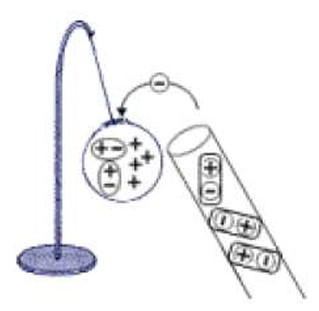
\includegraphics[width=8cm]{Images/img2.jpg}
	\caption{Cuerpos en estado cargado y neutro, eléctricamente.}\label{Fig:fg2}
\end{figure}

\begin{figure}[H]
	\centering
	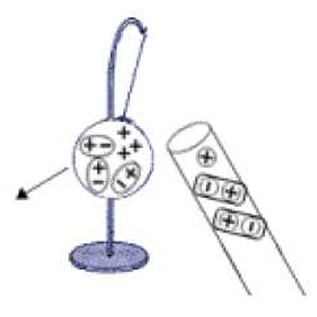
\includegraphics[width=8cm]{Images/img3.jpg}
	\caption{Cuerpos después de la acción por contacto.}\label{Fig:fg3}
\end{figure}
% ------------------------------------------------------------------------------------------
\subsubsection{Por Inducción}
Al acercar un cuerpo cargado al conductor neutro, las cargas eléctricas se
mueven de tal manera que las de signo igual a las del cuerpo cargado se alejan
en el conductor y las de signo contrario se aproximan al cuerpo cargado,
quedando el conductor polarizado.
%==========================================================================================
\section{Equipos y Materiales}
\begin{enumerate}[label=\itemcirccz{azzul}{\alph*},itemsep=2pt,partopsep=6pt]
	\item Franela.
	\item Lapiz, lapicero.
\end{enumerate}

% \begin{multicols}{2}
% 	\setlength{\columnseprule}{0pt}
% 	\begin{figure}[H]
% 		\centering
% 		%\caption{Dinamómetro}
% 		\includegraphics[width=2.5cm]{Images/Image_iii.jpeg}
% 	\end{figure}

% 	\begin{figure}[H]
% 		\centering
% 		\includegraphics[width=7cm]{Images/Image_iv.jpeg}
% 		\caption{Vaso precipitado}
% 	\end{figure}

% 	\begin{figure}[H]
% 		\centering
% 		\includegraphics[width=7.5cm]{Images/Image_v.jpeg}
% 		\caption{Calorímetro.}
% 	\end{figure}
% \end{multicols}
%==========================================================================================
\section{Procedimiento Experimental}
\subsection{Frotamiento}
Frotamiento de un lápiz al cabello o casaca, al acercarle al material más
liviano como es el papel se observará como el papel es atraído al lápiz, esto
ocurre porque el lapiz dejo de ser una carga neutra al frotarse con el cabello.
\subsection{Contacto}
Como podemos observar en la \textbf{Fig. 2} tenemos una esfera cargada
eléctricamente y al lado izquierda de la esfera otro cuerpo cilíndrico que está
en estado neutro para tener una de las formas de electrización del cuerpo en
este caso por contacto como su propio nombre lo indica tenemos que hacer rozar
o tocar los dos cuerpos en el siguiente observaremos.

Después del contacto de ambos cuerpos en la \textbf{Fig. 3} notamos, que la
esfera ganó electrones, este es uno de los casos de las 3 formas de
electrización que existen a consecuencia del frotamiento.
\subsection{Inducción}
\begin{figure}[H]
	\centering
	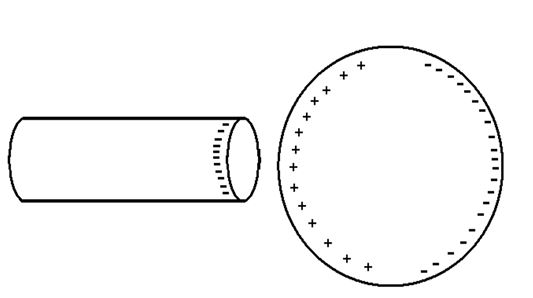
\includegraphics[width=10cm]{Images/img4.JPG}
	\caption{Barra cargada que se acerca a un cuerpo conductor produciendo una redistribución de cargas sobre su superficie.}\label{}
\end{figure}
\begin{figure}[H]
	\centering
	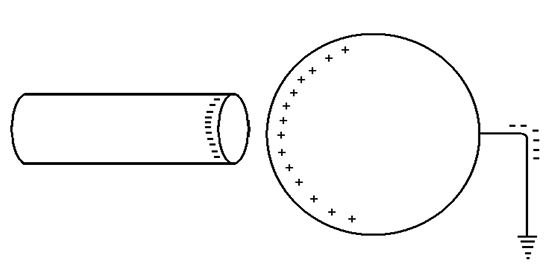
\includegraphics[width=10cm]{Images/img5.JPG}
	\caption{Cuando se pone a tierra el extremo del opuesto del cuerpo conductor las cargas negativas van a tierra dejando el cuerpo cargado sin contacto con la barra.}\label{}
\end{figure}
\subsection{Polarización}
\begin{figure}[H]
	\centering
	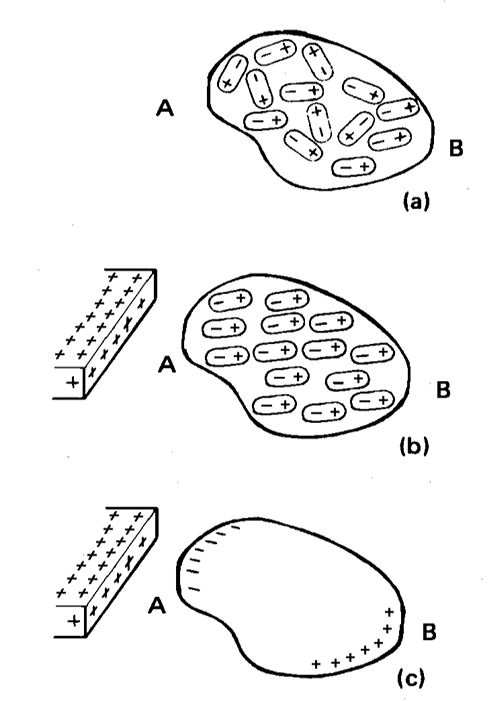
\includegraphics[width=8cm]{Images/img6.JPG}
	\caption{Material dieléctrico constituido por moléculas polares orientadas al azar (a), cuando se apr oxima una barra cargada las moléculas tienen una pequeña reorientación (b), en esas condiciones los extremos del signo material quedan cargados con cargas de distinto. Cuando se aleja la barra el sistema retoma la configuración original.}
\end{figure}
% \begin{dyNoteImportant}[morado01!20]{azulfor!10}{black!80}{Procedimientos}
% 	\begin{itemize}[label=\textbf{$\bullet$},itemsep=2pt,partopsep=6pt]
% 		\item Arme el equipo como se muestra en la figura.
% 		\item Calienta la miuestra de masa $m$ y calor específico $c$ a $T_1$, sumergido en
% 		      el agua en ebullición.
% 		\item Sumerge la muestra en agua fría de masa $M$ que contiene un calorímetro de masa
% 		      $M'$ y de calor específico $c'$.
% 	\end{itemize}
% \end{dyNoteImportant}
% \subsection{Para el Agua}
% \begin{enumerate}[label=\bfseries\alph*.-,itemsep=2pt, partopsep=6pt]
% 	\item \textbf{Calculando el equivalente en agua del calorímetro}
% 	      \[k=\cfrac{m(T-T_e)}{T_e-T_0}-M\]
% 	      Reemplzando:
% 	      \[k=\cfrac{200(91-54)}{54-18.5}-120\]
% 	      Finalmente:
% 	      \[k=88.54\]
% 	\item \textbf{Calculando el calor específico del sólido}
% 	      \[c=\cfrac{(M+k)(T_e-T_0)}{m\cdot(T-T_e)}\]
% 	      Reemplzando:
% 	      \[c=\cfrac{(120+k)(54-18.5)}{200\times(91-54)}\]
% 	      Finalmente:
% 	      \[c=1.000\,\,4\]
% \end{enumerate}
%==========================================================================================
% \section{Procesamiento de Datos Experimentados}
%==========================================================================================
\section{Tabla de Comparación}
\begin{table}[H]
	\centering
	\begin{tabular}{L{2.2cm}L{3.5cm}L{5.3cm}C{3cm}}
		\rowcolor{gray!10}Método & Requisitos                                                                        & Características                                                                                                                                                        & Material                                                      \\
		Frotamiento              & Movimiento relativo entre los cuerpos. Los cuerpos neutros.                       & Hay transferencia de carga. Un cuerpo queda con carga negativa y el otro con carga positiva Cada cuerpo queda con carga neta diferente de cero.                        & Aislantes, conductores siempre y cuando se aísle previamente. \\
		Inducción                & Un cuerpo previamente cargado. Separados pero cerca.                              & No hay transferencia de carga. No siempre la carga neta del conductor es cero.                                                                                         & Metales.                                                      \\
		Polarización             & Un cuerpo previamente cargado. Separados pero cerca.                              & No hay transferencia de carga. Siempre la carga neta del material aislante es cero.                                                                                    & Aislantes.                                                    \\
		Contacto                 & Un cuerpo previamente cargado. Se requiere contacto físico entre los dos cuerpos. & Hay transferencia de carga. El proceso de transferencia se da hasta que se logra el equilibrio electrostático, los dos cuerpos quedan con el mismo potencial eléctrico & Aislantes y conductores.                                      \\
	\end{tabular}
\end{table}
%==========================================================================================
\section{Conclusiones}
\begin{itemize}[label=\textbf{$\bullet$},itemsep=2pt,partopsep=6pt]
	\item Los cuerpos, en principio, se encuentran en estado eléctricamente neutro. Para
	      que un cuerpo se cargue es preciso que pierda o gane electrones.
	\item Electrización por frotamiento: consiste en frotar un cuerpo con otro. Los
	      electrones pasan de uno de ellos (que queda cargado positivamente) al otro (que
	      queda cargado negativamente).
	\item Electrización por inducción: cuando aproximamos un cuerpo cargado a otro en
	      estado neutro, todas las cargas de signo contrario al cargado se aproximarán a
	      éste, debido a que las cargas de distinto signo se atraen.
	\item Electrización por contacto: cuando un cuerpo tiene un exceso de carga de un
	      signo y se pone en contacto con un cuerpo eléctricamente neutro, pueden pasar a
	      éste cargas del primero. Decimos que se ha cargado por contacto.
\end{itemize}
%==========================================================================================